%\usepackage[latin1]{inputenc}
%\usepackage{amsmath}
%\usepackage{amsfonts}
%\usepackage{amssymb}
%\usepackage[active]{srcltx} %for kdvi and kile
%\usepackage{epsfig}         %for the figures
%\usepackage{verbatim}       %for the comment-environment

%\newtheorem{example}{Example}

%\newenvironment{code}{\begin{verbatim}}{\end{verbatim}}
  
  
\section{Example: A triangle and its altitudes}
    We want to create an applet which draws a triangle with three moveable 
    points and computes the altitudes.
    
    \subsection*{The canvas}
      Generally for any visualization we need a so called "canvas" (or several 
      of them) to draw our objects of visualization. The \appfac for this 
      purpose provides different predefined canvases, such as a single or a 
      side-by-side canvas for both Graphics2D or Java3D applets. Any applet 
      therefore shall extend one of the abstract classes 
      \begin{itemize}
        \item \verb SingleG2DCanvasApplet ,
        \item \verb SideBySideG2DCanvasApplet ,
        \item \verb SingleJ3DCanvasApplet , or
        \item \verb SideBySideJ3DCanvasApplet . 
      \end{itemize}
      There is also an an applet skeleton for pure symbolic displaying with no 
      canvas, the \verb NoCanvasApplet .
      
    \subsection*{The methods init() and initializeObjects()}
      The method \verb init()  is called from the applet context (i.e. the browser or appletviewer) 
      or by a wrapper-main method (don`t forget, your applet won't work otherwise!). It calls at least 
      the method \verb initializeObjects(),  and adds all created 
      objects to the canvas.

      With an empty implementation,  we can already have a look at our efforts 
      (see below) until now. As can be seen, some control 
      icons are automatically added as well as a standard \mbox{"help"-button}. 
        \begin{footnotesize}
        \begin{verbatim}
import net.mumie.mathletfactory.appletskeleton.g2d.SingleG2DCanvasApplet;
import net.mumie.mathletfactory.util.BasicApplicationFrame;

public class TriangleAltitude extends SingleG2DCanvasApplet{
  
  public void init() {
    super.init();
    setTitle("Triangle Altitude Applet");
    initializeObjects();
  }
  
  protected void initializeObjects(){
  }

  public static void main(String[] args){
    TriangleAltitude myApplet = new TriangleAltitude();
    myApplet.init();
    BasicApplicationFrame f = new BasicApplicationFrame(myApplet,500);
    f.pack();
    f.setVisible(true);
  }
}
        \end{verbatim}
        \end{footnotesize}
        \begin{center}
	  \resizebox*{7cm}{!}{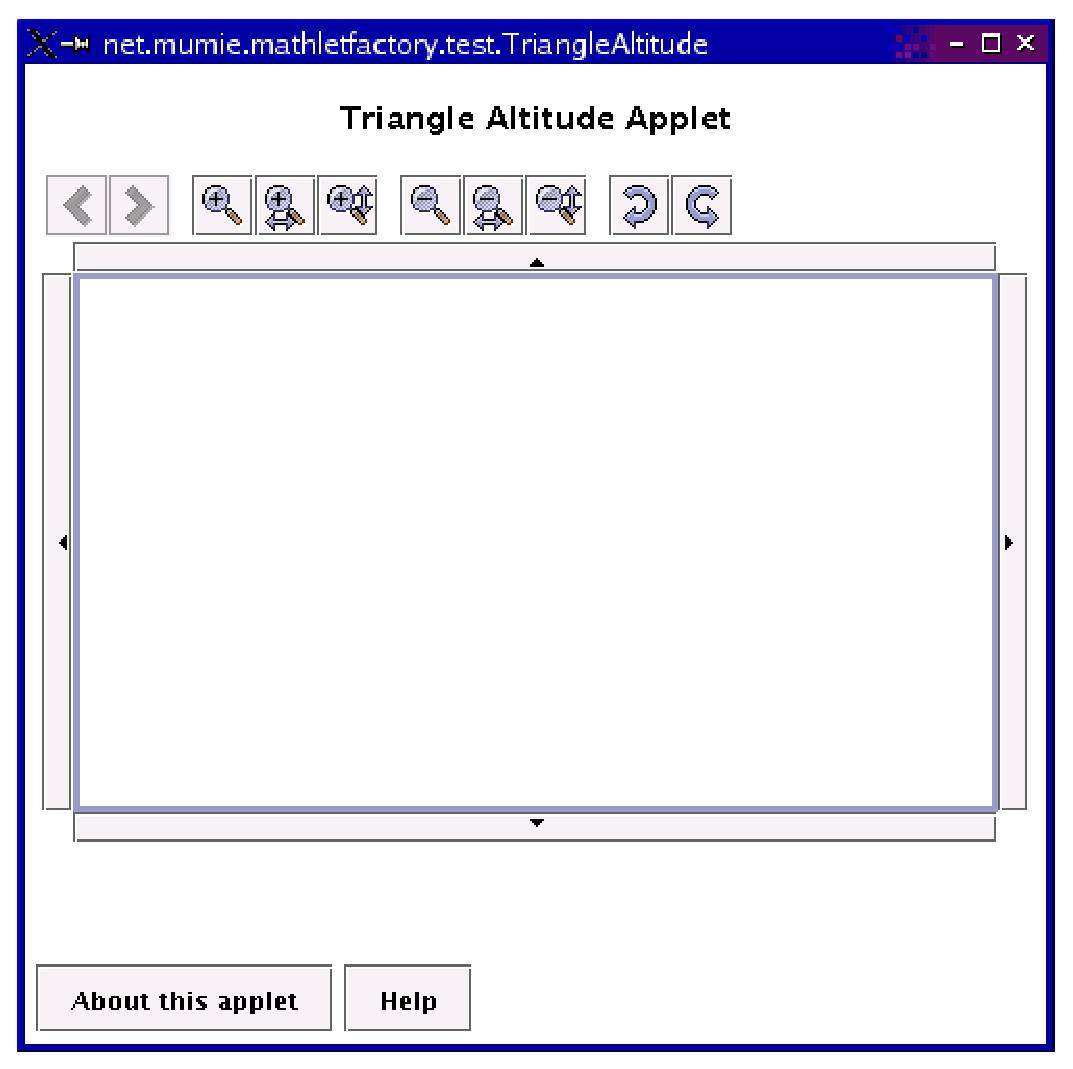
\includegraphics{images/triangleAltitudeFirst}}\\
        {\sf A single canvas applet.}\\
        \label{singlecanvas}
        \end{center}
    \subsection*{Number classes}
      Almost all objects are based on a so called number class like 
      \verb MDouble ,  \verb MRational ,  \verb MInteger ,  or 
      \verb MComplex .  They represent the real (with IEEE \verb double  precision), rational, natural, or complex 
      numbers. All computations are done within this class.
    \subsection*{Affine2DPoints}
      For the triangle we need three points A, B, C. They are realized by a so called 
      \verb MMAffine2DPoint  and defined by the representing number class and the coordinates:
      \begin{footnotesize}
      \begin{verbatim}
A = new MMAffine2DPoint(MDouble.class, -0.3, 0.3);
B = new MMAffine2DPoint(MDouble.class, 0.25, 0.25);
C = new MMAffine2DPoint(MDouble.class, -0.25, -0.25).
      \end{verbatim}
      \end{footnotesize}
      \vspace{-0.8cm}
    \subsection*{MouseTranslateHandler and KeyboardTranslateHandler}
      Since we want the points to be moveable by mouse and keyboard we create a
      so called \verb Affine2DMouseTranslateHandler  and an 
      \verb Affine2DKeyboardTranslateHandler  and add them to the points:
      \begin{footnotesize}
      \begin{verbatim}
amth = new Affine2DMouseTranslateHandler(getCanvas());
akth = new Affine2DKeyboardTranslateHandler(getCanvas());
A.addHandler(akth);     A.addHandler(amth);
B.addHandler(akth);     B.addHandler(amth);
C.addHandler(akth);     C.addHandler(amth);
      \end{verbatim}
      \end{footnotesize}
      \vspace{-0.8cm}
    \subsection*{Affine2DLineSegments}
      Now we need some line segments to connect the points of the triangle:
      \begin{verbatim}
AB = new MMAffine2DLineSegment(A,B);
BC = new MMAffine2DLineSegment(B,C);
CA = new MMAffine2DLineSegment(C,A).
      \end{verbatim}
      \vspace{-0.3cm}
      We also need line segments which represent the altitudes:
      \begin{verbatim}
altitude_AB = new MMAffine2DLineSegment(C,getPerpendicularFoot(A,B,C));
altitude_BC = new MMAffine2DLineSegment(A,getPerpendicularFoot(B,C,A));
altitude_CA = new MMAffine2DLineSegment(B,getPerpendicularFoot(C,A,B)).
      \end{verbatim}
      \vspace{-0.3cm}
      The method \verb getPerpendicularFoot()  returns a 
      \verb MMAffine2DPoint  representing the footpoint of the altitude.
      Some mathematical computation is
      done within this method which is not of interest for us now.

      Maybe the footpoint of an altitude does not lie on an edge of the 
      triangle. So we extend the edges by another line segment:
      \begin{footnotesize}
      \begin{verbatim}
aFootC = new MMAffine2DLineSegment(A,getPerpendicularFoot(A,B,C));
bFootC = new MMAffine2DLineSegment(B,getPerpendicularFoot(A,B,C));
bFootA = new MMAffine2DLineSegment(B,getPerpendicularFoot(B,C,A));
cFootA = new MMAffine2DLineSegment(C,getPerpendicularFoot(B,C,A));
cFootB = new MMAffine2DLineSegment(C,getPerpendicularFoot(C,A,B));
aFootB = new MMAffine2DLineSegment(A,getPerpendicularFoot(C,A,B)).
      \end{verbatim}
      \end{footnotesize}
      \vspace{-0.8cm}
      
%%%%%%%%%%%%%%%%%%%%%%%%%%%%%%%%%%%%%%%%%%%%%%%%%%%%%%%%%%%%%%%%%%%%%%%%%%%%%%%%%%%%%%%%%%%%%%%%
    \subsection*{Add objects to the canvas}
      Now all objects are created we have to add them to the canvas:\\\\
\begin{tabular}{l|l}
\begin{minipage}{6.5cm}
\begin{footnotesize}
\begin{verbatim}
getCanvas().addObject(A);
getCanvas().addObject(B);
getCanvas().addObject(C);

getCanvas().addObject(altitude_AB);
getCanvas().addObject(altitude_BC);
getCanvas().addObject(altitude_CA);
\end{verbatim}
\end{footnotesize}
\end{minipage}
&\begin{minipage}{6cm}
\begin{footnotesize}
\begin{verbatim}
getCanvas().addObject(AB);
getCanvas().addObject(BC);
getCanvas().addObject(CA);

getCanvas().addObject(aFootC);
getCanvas().addObject(bFootC);
getCanvas().addObject(cFootA);
getCanvas().addObject(cFootB);
getCanvas().addObject(aFootB);
getCanvas().addObject(bFootA);
\end{verbatim}
\end{footnotesize}
\end{minipage}
\end{tabular}
      
%%%%%%%%%%%%%%%%%%%%%%%%%%%%%%%%%%%%%%%%%%%%%%%%%%%%%%%%%%%%%%%%%%%%%%%%%%%%%%%%%%%%%%%%%%%%%%%%
    \subsection*{Display Properties}
      As can be seen in figure ??? all the lines and points have the standard 
      color black. If we want to give them another color we have to define
      \verb PointDisplayProperties   and \verb LineDisplayProperties  and set 
      them for the points and lines:
      \begin{footnotesize}
      \begin{verbatim}
private PointDisplayProperties pp = new PointDisplayProperties();
private LineDisplayProperties ll = new LineDisplayProperties();
private LineDisplayProperties mm = new LineDisplayProperties();
private LineDisplayProperties kk = new LineDisplayProperties();

\end{verbatim}
\end{footnotesize}
\begin{tabular}{l|l}
\begin{minipage}{7cm}
\begin{footnotesize}
\begin{verbatim}

pp.setObjectColor(Color.blue);
ll.setObjectColor(Color.red);
mm.setObjectColor(Color.red);
mm.setFilled(false);
kk.setObjectColor(Color.yellow);

A.setDisplayProperties(pp);
B.setDisplayProperties(pp);
C.setDisplayProperties(pp);

altitude_AB.setDisplayProperties(kk);
altitude_BC.setDisplayProperties(kk);
altitude_CA.setDisplayProperties(kk);

\end{verbatim}
\end{footnotesize}
\end{minipage}
&\begin{minipage}{6cm}

\begin{footnotesize}
\begin{verbatim}

AB.setDisplayProperties(ll);
BC.setDisplayProperties(ll);
CA.setDisplayProperties(ll);

aFootC.setDisplayProperties(mm);
bFootC.setDisplayProperties(mm);
bFootA.setDisplayProperties(mm);
cFootA.setDisplayProperties(mm);
cFootB.setDisplayProperties(mm);
aFootB.setDisplayProperties(mm);

\end{verbatim}
\end{footnotesize}
\end{minipage}
\end{tabular}
    
The result can be seen in figure ??. 

%%%%%%%%%%%%%%%%%%%%%%%%%%%%%%%%%%%%%%%%%%%%%%%%%%%%%%%%%%%%%%%%%%%%%%%%%%%%%%%%%%%%%%%%%%%%%%%%
    \subsection*{Dependency}
      Now our points are moveable but the lines do not move with them. 
      Obviously the position of the lines depend on the position of the points.
      This is described by a so called \verb DependencyAdapter  and the 
      method \verb dependsOn().  For example for the edges of the triangle we 
      have
      \begin{footnotesize}
      \begin{verbatim}
DependencyAdapter DPA = new DependencyAdapter() {
  public void doUpdate(MMObjectIF dependant, MMObjectIF[] free) {
    MMAffine2DLineSegment line = (MMAffine2DLineSegment) dependant;
    line.setInitialPoint((MMAffine2DPoint)free[0]);
    line.setEndPoint((MMAffine2DPoint)free[1]);
  }
};
AB.dependsOn(new MMObjectIF[]{A,B},DPA);
BC.dependsOn(new MMObjectIF[]{B,C},DPA);
CA.dependsOn(new MMObjectIF[]{C,A},DPA);
      \end{verbatim}
      \end{footnotesize}
      \vspace{-0.3cm}
      Hereby the first argument \verb new  \verb MMObjectIF[]{A,B}  of the 
      method \verb dependsOn()  is an array of objects on which the object 
      \verb AB  depends. This array is passed to the 
      method \verb doUpdate  in the \verb DependencyAdapter  \verb DPA  as 
      parameter \verb free.  \verb AB  is passed to the 
      method \verb doUpdate  in the \verb DependencyAdapter  as parameter 
      \verb dependent.  \verb doUpdate  describes the action to perform when
      an object of the array \verb free  is changed.
    \subsection*{Reset, Screenshot, About this applet button}
      With the commands
      \begin{verbatim}
addResetButton();
addScreenShotButton();
      \end{verbatim}
      \vspace{-0.3cm}
      we can add a reset and a screenshot button. The functionality of the 
      reset button is defined in the method \verb reset(),  which calls the 
      method \verb initializeObjects()  and repaints the canvas:
      \begin{footnotesize}
      \begin{verbatim}
public void reset(){
  initializeObjects();
  getCanvas().renderScene();
  getCanvas().repaint();
}.
      \end{verbatim}
      \end{footnotesize}
      \vspace{-0.3cm}
    A HTML-description of the functionality of the applet can be saved in a 
    file with the name \verb <class_name>_info.html. This desciption is opend 
    in another window by clicking the about-this-applet button.\\

    \begin{center}
	\resizebox*{6cm}{!}{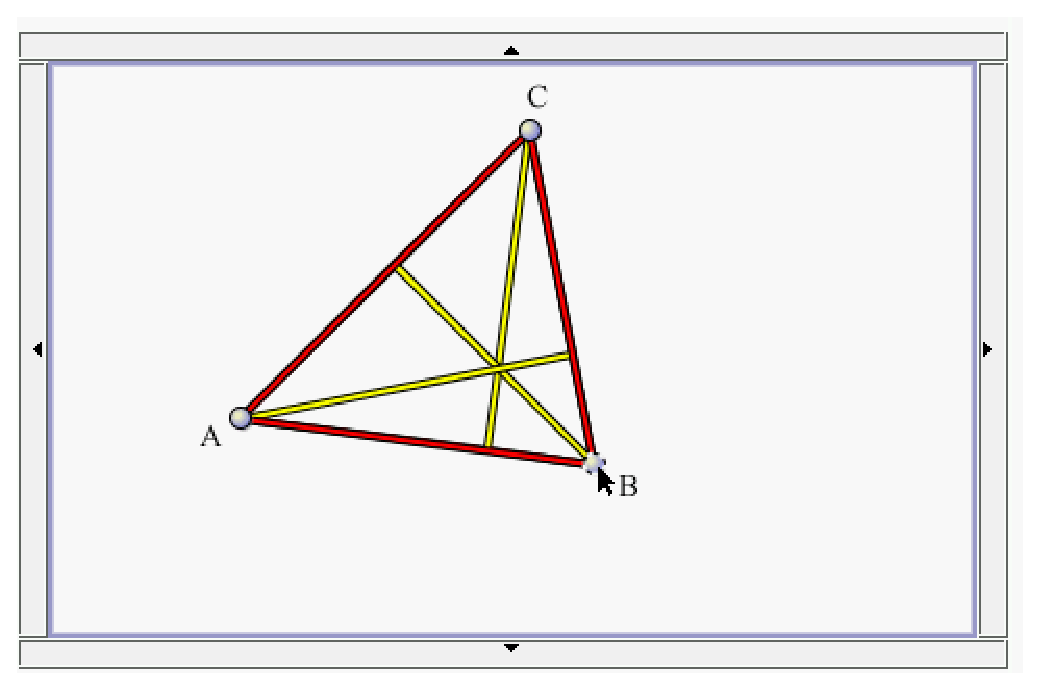
\includegraphics{images/triangle_altitudes}}\\
	{\sf The completed applet}
    \end{center}
    Now our first applet is ready. The full program can be found in the Appendix (TriangleAltitude).

%%%%%%%%%%%%%%%%%%%%%%%%%%%%%%%%%%%%%%%%%%%%%%%%%%%%%%%%%%%%%%%%%%%%%%%%%%%%%%%%%%%%%%%%%%%%%%%%
	\subsection*{Summary: Building Mathlets}
	\label{building_mathlets}
	These examples should illuminate the process of rapid applet development. The linear process 
	model we used can be generalized to the following steps:
	
	\begin{enumerate}
	\item Choose the display type and numbers of displays to be used and extend the corresponding applet skeleton.
	\item Add the chosen mmobjects and their iconic or symbolic representations
	\item Add necessary handlers
	\item Create the update graph by adding updaters and creating dependencies
	\end{enumerate}

